\chapter{New Proposals}\label{ch:NewProposals}

Finding the optimal partition in a dataset according to any kind of reasonable criteria is known to be a $\mathbf{NP}$-hard problem. As we have already mentioned in Section \ref{sec:FeasibilityProblem}, the use of constraints may modify the complexity of the clustering problem, making it $\mathbf{NP}$-complete and therefore intractable \cite{davidson2005clustering}. Bearing this in mind, in this chapter we propose two new approaches to find approximate solutions to the constrained clustering problem. In Section \ref{sec:CCSHADE} a \acf{DE} based approach is presented, while in Section \ref{sec:DILS} a new \acf{LS} variant is discussed, as well as its application to constrained clustering.


\section{Constrained Clustering Through Differential Evolution} \label{sec:CCSHADE}

The constrained clustering problem can be formulated in terms of optimization, so that we can apply various optimization techniques to solve it. As mentioned earlier, it is a difficult problem to solve, so nature-inspired techniques are presented as a promising option to find quality approximate solutions. Nature is the best example of adaptive problem solving since it can apply an optimal strategy suited for each natural phenomenon \cite{fausto2019ants}. Nature-inspired algorithms are designed to emulate natural optimization phenomena, such as evolution, collective behavior of animals, physics laws or even human being-related processes. There have been attempts to solve the constrained clustering problem with nature-inspired algorithms, such as the adaptation of the \acf{BRKGA} presented in \cite{de2017comparison}. Swarm-based methods have also been applied to constrained clustering, such as the one presented in \cite{xu2013improving}.

\acs{DE} is an evolution-based algorithm that has proven to be excellent in real-domain problem solving \cite{das2011differential}. In this section we propose the first \acs{DE} application to find quality solutions for the constrained clustering problem. In particular, we will take as basis for our proposal one of the \acs{DE} variants which showed excellent behavior in worldwide competitions, known as \acs{SHADE} \cite{molina2018insight}. We will make use of the Random-key concept from \acs{BRKGA}, along with proposing a new fitness function, to build the already mentioned \acs{DE} application.

\subsection{A Glimpse into Differential Evolution}

Evolution-based methods comprise a group of algorithms developed on the basis of the natural laws of evolution. In this type of techniques a population of individuals---representing potential solutions to the problem---is usually employed, which compete and combine through a certain number of generations so that the population evolves in such a way that only the best individuals, and thus the best solutions, remain at the end. This type of techniques involves the development of a series of operators that allow us to simulate the evolution process, such as crossover, mutation and selection operators \cite{fausto2019ants}. 

\acf{DE}, which emerged in \cite{storn1997differential}, is a good example of evolution-based methods. From that point on, the reputation of \acs{DE} was consolidated in conferences and competitions where it was able to obtain competitive results that rivaled those achieved by the state-of-the-art. In particular, \acs{DE} excelled in real-coded optimization problems. A highly detailed analysis of \acs{DE} and its variants can be found in \cite{das2011differential}.

\acs{DE} arose as a variant of population-based evolutionary algorithms, its goal being to perform an intelligent search in the solution space of the problem in the most optimized and effective way possible.

Like most evolutionary algorithms, \acs{DE} uses a population of individuals $P$, where each individual $p_i$ is a vector of real values $p_i = \{p_{[i,1]},\cdots,p_{[i,v]}\}$, with $v$ being the number of features of each individual. Each $p_i$ serves as parameter for the function to be optimized. These individuals are considered solutions to the problem.

To guide the optimization process, we use a fitness function $f(\cdot)$. The task of \acs{DE} is to seek the parameter vector $p_i^*$ that minimizes a function such that $f(p_i)(f: \Omega \subseteq \mathfrak{R}^{v} \rightarrow \mathfrak{R})$, where $f(p_i^*) < f(p_i)$ for all $p_i \in \Omega$ with $\Omega$ a nonempty finite set that is the search domain.

\begin{figure}[!h]
	\centering
	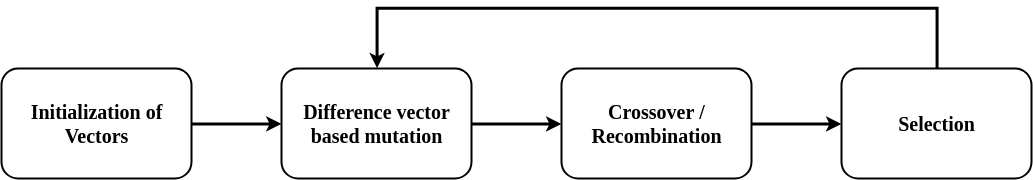
\includegraphics[scale=0.3]{gfx/NewProp/SHADE/DEop.png}
	\caption[The optimization process of \acs{DE}.]{The optimization process of \acs{DE} \cite{das2011differential}.}\label{fig:DE}
\end{figure}

The optimization process of \acs{DE} the works through a simple cycle of stages, presented in Figure \ref{fig:DE}, that we can summarize as follows:

\begin{itemize}
	
	\item \textbf{Initialization of Vectors}: \acs{DE} begins with a randomly initialized population of a given number of $v$-dimensional arrays of parameters. These vectors constitute candidate solutions for the problem to be solved.
	
	\item \textbf{Difference-vector-based mutation}: \acs{DE} introduces diversity into the population via the mutation operator. This operator is applied to each individual of the population, known in this context as the parent vector. It combines the parent vector with two randomly selected vectors from the population by applying an arithmetic operator to them. The result of this process is a mutant vector.
	
	\item \textbf{Crossover/Recombination}: The mutant vector exchanges some components with its associated parent to form a trial vector, which will be the candidate to replace the parent vector. Several strategies exist to generate this trial vector, which we will not delve into; however, they can be found in \cite{das2011differential}.
	
	\item \textbf{Selection}: The newly generated trial vector is compared with its associated parent using the fitness function. If the trial vector is better than the parent, then it will replace the parent in the next generation. It is worth noting that, following this strategy, the population never degenerates but only gets better or remains the same.
	
\end{itemize}

Even though \acs{DE} was a major breakthrough in terms of real optimization, many variants have been developed since its invention that provide better results. We will focus on the \acs{SHADE} variant, which adaptively optimizes some of the parameters of \acs{DE}. To carry out this task \acs{SHADE} uses a historic record of values for these parameters that allows it to set them in favor of the optimization process, based on how good the algorithm behaved with certain parameter values in the past (see Section \ref{sec:SHADE}).

\subsection[Brief Review of the \acsfont{BRKGA} Algorithm]{Brief Review of the BRKGA Algorithm} \label{sec:brkga}

\acp{GA} emerged as one of the first metaheuristics inspired by the concept of natural selection and evolution. It is one of the most studied and successful evolutionary algorithms, thanks in part to its simplicity and ease of implementation \cite{fausto2019ants, goldberg1989genetic}. 

In a \acs{GA}, a population $P$ of a given number of solutions \sloppy $p_i = \{p_{[i,1]}, \cdots, p_{[i,v]}\}$ is first initialized; these solutions are also called chromosomes or individuals. Each element of a chromosome is called gene and the value it takes is known as allele. To simulate the natural processes of evolution and natural selection, the set of evolutionary operators that \acsp{GA} make use of is similar to that used by \acs{DE}: crossover, mutation and selection. The crossover operator consists in combining two different chromosomes (parents) from the population and obtaining a new chromosome (offspring) which inherits alleles for its genes from both parents. The mutation operator is used by \acsp{GA} to avoid local optima, and it consists in introducing random changes into the population to favor diversity. The selection operator is used to determine whether a chromosome is suitable to survive for the next generation, and to accomplish this task it employs a fitness function $f(\cdot)$ that assigns a value to each chromosome to assess its quality as a solution for the problem. \acsp{GA} apply these operators through a series of generations to hopefully obtain a solution for the problem to solve that is close to the optimal \cite{fausto2019ants}.  

\acf{RKGA} emerged in \cite{bean1994genetic} as a solid approach to highly constrained problems. It uses vectors of random numbers to represent solutions to the problem (individuals) which are used as keys to obtain the actual solutions. Random-key vectors are sampled from the space $[0,1]^{v}$, which is used as a surrogate space for the literal solution space. Points in the random-key space are transferred to the literal solution space via a decoder for fitness evaluation. A decoder is a deterministic procedure that allows us to map random-key vectors to the literal solution space. We can build a decoder that always provides as a result a feasible solution to the problem we want to solve, thus avoiding the feasibility problem that we found in classic \acsp{GA}.

The \acf{BRKGA} was first proposed in \cite{gonccalves2011biased} as a variant of the \acs{RKGA}. In the \acs{BRKGA} optimization process, first, the population $P$ of $|P|$ vectors of random-keys is initialized; this will be the initial generation. Each random-key vector $p_i$ has $v$ random-keys in it. The population is sorted by the fitness value $f(p_i)$ of each individual to select the first $P_e$ individuals, this is, the elite of the population. The elite will be preserved in the next generation without modification. To introduce diversity, a number $P_m$ of new random-keys vectors are also included in the next generation. The remaining individuals of the new generation ($|P| - P_e - P_m$) are obtained through crossovers between elite and non-elite parents.

It should be noted that in \acs{BRKGA} there is a clear differentiation between problem-dependent and problem-independent elements. The independent part of the algorithm has no knowledge of the problem it solves, it is limited to performing the operations related to the population optimization process. The dependent part of the problem is composed of the decoder and the fitness function, which allow us to obtain actual solutions for the problem and its evaluation. Therefore, to specify a \acs{BRKGA} optimization scheme it is only necessary to define the decoder and the fitness function \cite{gonccalves2011biased}.

\subsection[\acsfont{BRKGA} Optimization Scheme for Constrained Clustering]{BRKGA Optimization Scheme for Constrained Clustering} \label{sec:AdaptationofBRKGA}

An adaptation of \acs{BRKGA} for constrained clustering was proposed in \cite{de2017comparison}, we will refer to it as \acs{BRKGA}$_{CC}$.

In this scheme each random-key vector has $n$ random-keys in it ($v = n$). The decoder divides the interval $[0,1]$ in $k$ intervals, so there exists a correspondence between each random-key (instance $x_i$) and the integer (label $l_i$) corresponding to the interval which it lies in. Table \ref{tab:decodingrk} shows an example of random-key decoding for a dataset withteninstances ($n$ = 10) and $k = 3$. Note that extreme values 0 and 1 can also appear in a random-key vector.

\begin{table}[!h]
	\centering
	%\setlength{\arrayrulewidth}{1mm}
	\setlength{\tabcolsep}{7pt}
	\renewcommand{\arraystretch}{1.2}
	\resizebox{\textwidth}{!}{
		\begin{tabular}{|c|c|c|c|c|c|c|c|c|c|c|}
			\hline
			Index (instance) & 1 & 2 & 3 & 4 & 5 & 6 & 7 & 8 & 9 & 10 \\
			\hline
			Random-key & 0.12 & 0.37 & 0.66 & 0.56 & 0.00 & 0.97 & 0.23 & 0.25 & 0.15 & 1.00 \\
			\hline
			Cluster (label) & 1 & 2 & 2 & 2 & 1 & 3 & 1 & 3 & 1 & 3 \\
			\hline
			
	\end{tabular}}
	\caption[Random-key decodification example.]{Random-key decodification example \cite{de2017comparison}.}
	\label{tab:decodingrk}
\end{table}

Once the decoded solution has been obtained, the fitness value of the solution (individual $p_i$) is computed as in Equation \eqref{eq1}.

\begin{equation}
f_1(p_i) = z_i + \overbrace{(\mu * n * \text{infeasibility}_i)}^\text{penalty},
\label{eq1}
\end{equation}

\noindent where $\mu$ is a high value, $\text{infeasibility}_i$ is the number of non-satisfied constraints and $z_i$ is the within-cluster-sum-of-squares which can be computed as in Equation \eqref{eq2}.

\begin{equation}
z_i = \sum_{c_j \in C_i} \left[ \frac{\sum_{x_a, x_b \in c_j} d^2(x_a,x_b)}{|c_j|}\right],
\label{eq2}
\end{equation}

\noindent where $C_i$ is the partition of dataset $X$ defined by solution (individual) $p_i$, and $(x_a, x_b)$ are instances in the cluster $c_j$ such that $a \neq b$ and the Euclidean distance ($d^2(\cdot, \cdot)$) between each pair of instances in $C_i$ is included in the sum only once.

In \cite{de2017comparison}, the authors also added a new element to \acs{BRKGA}, an \acs{LS} procedure. This local optimization method is applied to each decoded individual in each generation, but its results are not transferred to the individual, so that diversity is maintained. Thus, the individuals produced by the \acs{LS} are only used to update the best solution found so far if needed. Figure \ref{fig:BRKGA_CC} shows a visual representation of the overall \acs{BRKGA} optimization process for constrained clustering. For more details on \acs{BRKGA}$_{CC}$ see \cite{de2017comparison}. Arrows in red indicate population sorting by fitness.

\begin{figure}[!h]
	\centering
	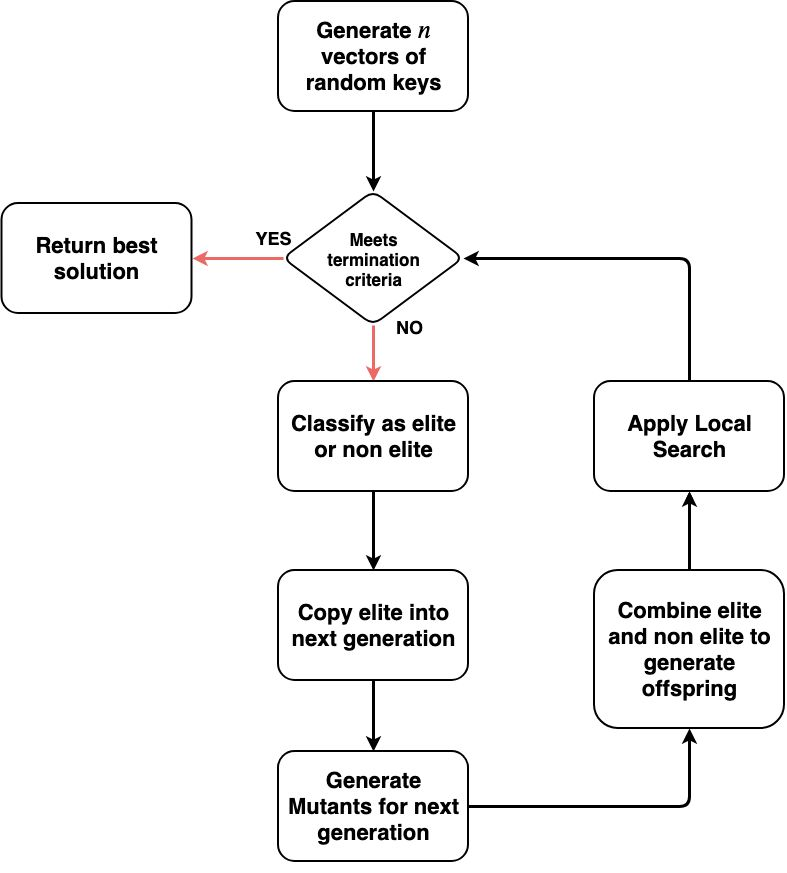
\includegraphics[scale=0.31]{gfx/NewProp/SHADE/BRKGA_Diagram.jpg} 
	\caption[\acs{BRKGA}$_{CC}$ optimization process for constrained clustering.]{\acs{BRKGA}$_{CC}$ optimization process for constrained clustering \cite{de2017comparison}.}\label{fig:BRKGA_CC}
\end{figure}

\subsection[The \acsfont{SHADE} Optimization Method]{The SHADE Optimization Method} \label{sec:SHADE}

\acf{SHADE} is an optimization method based on \acs{DE}. Proposed in \cite{tanabe2013success}, it was an improvement for the \acsfont{JADE} model, presented in \cite{zhang2009jade}.

Unlike \acsfont{JADE}, which only considers the parameters used in the previous generation, \acs{SHADE} uses a historical record of successful parameters as a mechanism for adapting parameters involved in the process of creating new generations.

Since \acs{SHADE} is an evolution-based algorithm, it shares elements with \acs{BRKGA} (Section \ref{sec:brkga}), so we will use a similar notation to define its elements. We will note the population as $P_G$, formed by $|P|$ individuals with the form $p_{[i,G]} = \{p_{[i,G,1]}, \cdots, p_{[i,G,v]}\}$, with $G$ indicating the generation to which $p_i$ belongs.

\subsubsection[\acsfont{SHADE} Operators]{SHADE Operators}

As in \acs{DE}, \acs{SHADE} employs mutant generation, crossover and selection operators to explore the space of solutions and bring in new generations of individuals.

The mutation strategy used by \acs{SHADE} is known as current-to-$p$best/1, and the expression that generates new individuals is described in Equation \eqref{eq3}.

\begin{equation}
m_{[i,G]} = p_{[i,G]} + F_i * (p_{[p\text{best}, G]} - p_{[i,G]}) + F_i * (p_{[r1, G]} - p_{[r2,G]}),
\label{eq3}
\end{equation}

\noindent where $m_{[i,G]}$ is the mutant vector, which is generated with an individual $p_{[i,G]}$ from the population serving as a starting point. Indices $r1$ and $r2$ are random values in the range $[0,|P|]$, different from $i$ and from each other. The individual $p_{[p\text{best}, G]}$ is randomly selected from among the best $|P| \times p\text{best}\;|\;p\text{best}\in [0,1]$ individuals in the population. This way, the parameter $p\text{best}$ controls the greediness of the mutation strategy. The parameter $F_i$ defines the magnitude of the operator.

After generating the mutant vector $m_{[i,G]}$, it is combined with the parent $p_{[i,G]}$ vector by means of a crossover operator; the result is the trial vector $t_{[i,G]} = \{t_{[i,G,1]}, \cdots, t_{[i,G,v]}\}$. \acs{SHADE} uses the Binomial crossover operator, which is defined by the Equation \eqref{eq4}.

\begin{equation}
t_{[i,G,j]} = \left\{ \begin{array}{lc}
m_{[i,G,j]} &   \text{if} \;\; \text{rand}[0,1) \le CR_i \;\; \text{or} \;\;j = j_{rand} \\
p_{[i,G,j]} &  \text{otherwise}
\end{array}
\right.,
\label{eq4}
\end{equation}

\noindent where $\text{rand}[0,1)$ is a random number selected from a normal distribution in the range $[0,1)$, $j_\text{rand}$ is a random integer selected from the range $[1,v]$, and $CR \in [0,1]$ is the crossover ratio.

The \acs{SHADE} selection operator determines the survivors individuals for the next generation. It compares each parent $x_{[i,G]}$ with the trial vector $t_{[i,G,j]}$, generated based on it. The best one of these two individuals will survive for the next generation. Equation \eqref{eq5} shows this concept.

\begin{equation}
p_{[i,G + 1]} = \left\{ \begin{array}{lc}
t_{[i,G]} &   \text{if} \;\; f(t_{[i,G]}) \le f(p_{[i,G]}) \\
p_{[i,G]} &  \text{otherwise}
\end{array}
\right..
\label{eq5}
\end{equation}

To maintain diversity, \acs{SHADE} can make use of an external archive $A$, in which parents $p_{[i,G]}$ who were replaced by their associated trial vector $t_{[i,G]}$ are saved. To make use of the archive, we will consider that the individual $p_{[r2,G]}$ from Equation \eqref{eq3} is selected from $P \cup A$. The archive size is the same as the population size. When the size of $A$ exceeds the size of $P$, random individuals are selected for removal to make room for new ones.

The parameters $p\text{best}$, $F_i$ and $CR_i$ are difficult to adjust and their selection is not trivial, as they largely determine the success of the optimization process. These are the parameters that \acs{SHADE} adaptively optimizes using the mentioned history record.

\subsubsection[\acsfont{SHADE} Parameter Adaptation Method]{SHADE Parameter Adaptation Method}

The \acs{SHADE} method stores in memory a structure $M$ with $|M|$ entries for parameters $F_i$ and $CR_i$, as shown in Table \ref{tab:SHADEmemory}. This structure is initialized with the value $0.5$ for all entries.

\begin{table}[!h]
	\centering
	%\setlength{\arrayrulewidth}{1mm}
	\setlength{\tabcolsep}{13pt}
	%\renewcommand{\arraystretch}{0.9}
	\resizebox{\textwidth}{!}{
		\begin{tabular}{|c|c|c|c|c|c|}
			\hline
			Index & 1 & 2 & $\cdots$ & $|M| - 1$ & $|M|$ \\
			\hline
			\hline
			$M_{CR}$ & $M_{[CR,1]}$ & $M_{[CR,1]}$ & $\cdots$ & $M_{[CR,|M|-1]}$ & $M_{[CR,|M|]}$ \\
			\hline
			$M_{F}$ & $M_{[F,1]}$ & $M_{[F,1]}$ & $\cdots$ & $M_{[F,|M|-1]}$ & $M_{[F,|M|]}$ \\
			\hline
			
	\end{tabular}}
	\caption[Historical memory $M_{CR}$, $M_{F}$ used by \acs{SHADE}.]{Historical memory $M_{CR}$, $M_{F}$ used by \acs{SHADE} \cite{tanabe2013success}.}
	\label{tab:SHADEmemory}
\end{table}

In each generation, parameters $CR_i$ and $F_i$ are calculated on the basis of the existing history by applying Equations \eqref{eq6} and \eqref{eq7}:

\begin{equation}
CR_i = \text{randn}_i(M_{[CR,r_i]}, 0.1),
\label{eq6}
\end{equation}

\begin{equation}
F_i = \text{randc}_i(M_{[F,r_i]}, 0.1),
\label{eq7}
\end{equation}

\noindent where $\text{randn}(\mu, \sigma^2)$ and $\text{randc}(\mu, \sigma^2)$ are random values from normal and Cauchy distributions respectively, with mean $\mu$ and variance $\sigma^2$. When a value for $CR_i$ outside of the range $[0,1]$ is generated, it is replaced by the corresponding limit value. If $F_i > 1$, then it is truncated to $1$; conversely, if $F_i < 0$, then Equation \eqref{eq7} is applied as many times as needed to obtain a legal value.

\acs{SHADE} keeps two auxiliary sets $S_{CR}$ and $S_F$ to store the $CR_i$ and $F_i$ values that were successfully used to generate a trial vector that replaced the parent. At the end of each generation, the content of the memory $M$ is updated following Equations \eqref{eq8} and \eqref{eq9}.

\begin{equation}
M_{[CR,h,G+1]} = \left\{ \begin{array}{lc}
\text{mean}_{WA} (S_{CR}) & \text{if} \;\; S_{CR} \neq \emptyset \\
M_{[CR,h,G]} &  \text{otherwise}
\end{array}
\right.,
\label{eq8}
\end{equation}

\begin{equation}
M_{[F,h,G+1]} = \left\{ \begin{array}{lc}
\text{mean}_{WL} (S_{F}) & \text{if} \;\; S_{F} \neq \emptyset \\
M_{[F,h,G]} &  \text{otherwise}
\end{array}
\right..
\label{eq9}
\end{equation}

The $h \;\; (0 \le h \le |M|)$ index specifies the position of the memory $M$ to be updated. This index is initialized to $0$ at the beginning of the optimization process and increased by one after every generation. When $h \ge |M|$ then $h$ is reset to 1. It is worth noting that, when there is a generation with no trial vectors successfully replacing their parents, no update of $M$ is done.

In Equation \ref{eq8}, the term $\text{mean}_{WA} (S_{CR})$ is the weighted mean, which is computed following Equations \eqref{eq10} and \eqref{eq11}, proposed in \cite{peng2009multi} to prevent $CR$ from converging to small values.

\begin{equation}
\text{mean}_{WA} (S_{CR}) = \sum_{i = 1}^{|S_{RC}|} \omega_i * S_{[RC,i]},
\label{eq10}
\end{equation}

\begin{equation}
\omega_i = \frac{\Delta f_i}{\sum_{i = 1}^{|S_{RC}|} \Delta f_i},
\label{eq11}
\end{equation}

\noindent where $\Delta f_i = |f(t_{[i,G]}) - f(p_{[i, G]})|$, which is the amount of improvement obtained from the trial vector with respect to the parent.

In Equation \ref{eq9} the term $\text{mean}_{WL} (S_{F})$ refers to the weighted Lehmer mean, which is computed as in Equation \eqref{eq12} (proposed in \cite{tanabe2013success}).

\begin{equation}
\text{mean}_{WL} (S_{F}) = \frac{\sum_{i = 1}^{|S_{F}|} \omega_i * S^2_{[F,i]}}{\sum_{i = 1}^{|S_{F}|} \omega_i * S_{[F,i]}}.
\label{eq12}
\end{equation}

Unlike parameters $S_{CR}$ and $S_F$, the parameter $p\text{best}$ from Equation \eqref{eq3}, used to set the greediness of the mutation strategy, is not included in the adaptive optimization process. However, it is not static: it is calculated for every individual $p_i$ of the population following Equation \eqref{eq13}.

\begin{equation}
p\text{best}_i = \text{randn}[2/N, 0.2],
\label{eq13}
\end{equation}

\noindent such that there is always at least two individuals to choose between.

\subsection[\acsfont{SHADE} Optimization Scheme for Constrained Clustering]{SHADE Optimization Scheme for Constrained Clustering} \label{sec:SHADEadapt}

In this section, we present an optimization scheme for the \acs{SHADE} algorithm when applied to constrained clustering. We will call this new approach \acs{SHADE}$_{CC}$. To begin with, we will use random-keys to create the individuals of the population; this way, each individual is defined as a vector of $n$ random-keys ($v = n$). Additionally, we will also make use of the initialization method and the decoder found in Section \ref{sec:AdaptationofBRKGA}. However, we propose a new fitness function to evaluate the quality of the individuals of the population, Equation \eqref{eq14}, whose element $z_i$ is obtained as in Equation \eqref{eq2}.

\begin{equation}
f_2(p_i) = z_i * (\text{infeasibility}_i + 1).
\label{eq14}
\end{equation}

Note that in Equation \eqref{eq14} no parameter is involved that cannot be calculated from the dataset or constraints, whereas in Equation \eqref{eq1} the $\mu$ parameter must be calculated and optimized for each individual problem. Therefore with Equation \eqref{eq14} a better generalization capability is obtained.

We found that with the fitness function defined in \eqref{eq1} there is no competition between the penalty term and the within-cluster-sum-of-squares term, because the penalty is always significantly larger than it or zero. This can bias the exploration of the solution space, restricting it in practice to those that satisfy all the constraints, even if the within-cluster-sum-of-squares is still improvable by moving two instances involved in a constraint to different clusters without violating that constraint.

With Equation \eqref{eq14} we try to find a trade-off between the within-cluster-sum-of-squares and the penalty term, allowing solutions that violate a certain number of constraints to compete with those who violate a smaller number of them but score a better within-cluster-sum-of-squares.

To make these concepts clear we consider a toy dataset and three partitions over it. The dataset from Figure \ref{fig:toydatasets} contains 100 instances and a single \acs{ML} constraint between two instances from the same class. Partitions $C_0$---displaying the true labels---and $C_1$ do not violate the constraint ($\text{infeasibility} = 0$), whereas $C_2$ does violate it ($\text{infeasibility} = 1$). However, $C_2$ shows a possibility, for later iterations, of adding both instances to their nearest cluster while also satisfying the \acs{ML} constraint.

\begin{figure}[bth]
	\myfloatalign
	{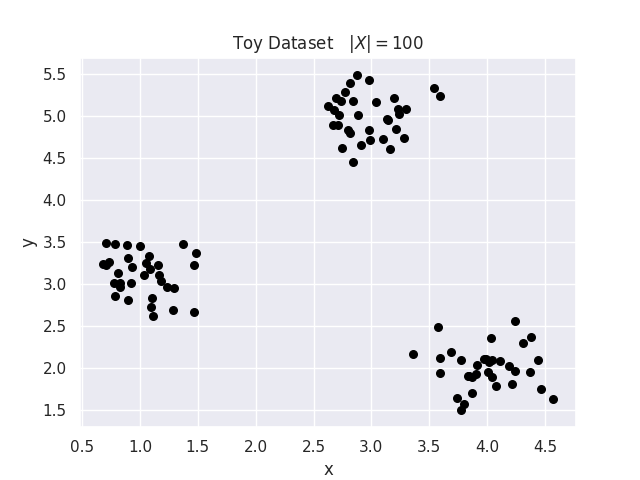
\includegraphics[width=.41\linewidth]{gfx/NewProp/SHADE/Dataset}} \quad
	%\subfloat[Imagen original]
	{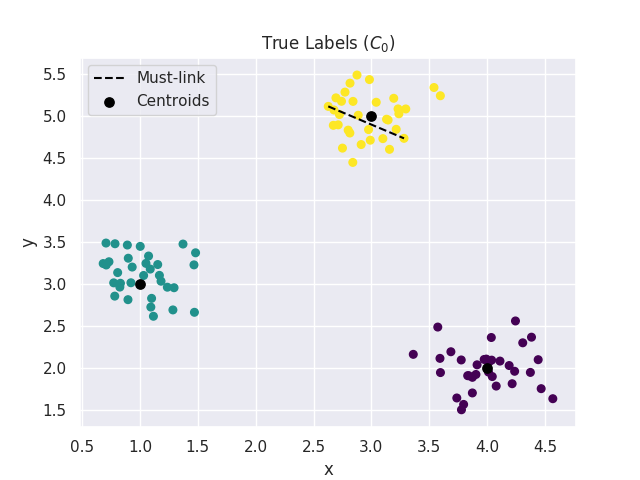
\includegraphics[width=.41\linewidth]{gfx/NewProp/SHADE/C0}} \quad
	%\subfloat[Clustering sin restricciones]
	{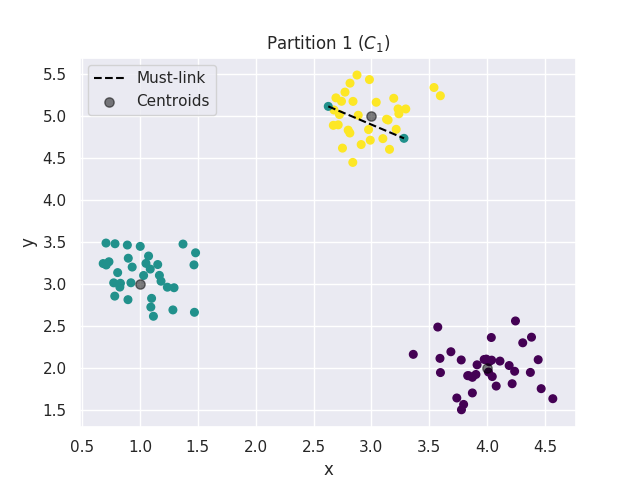
\includegraphics[width=.41\linewidth]{gfx/NewProp/SHADE/C1}} \quad
	%\subfloat[Clustering con restricciones]
	{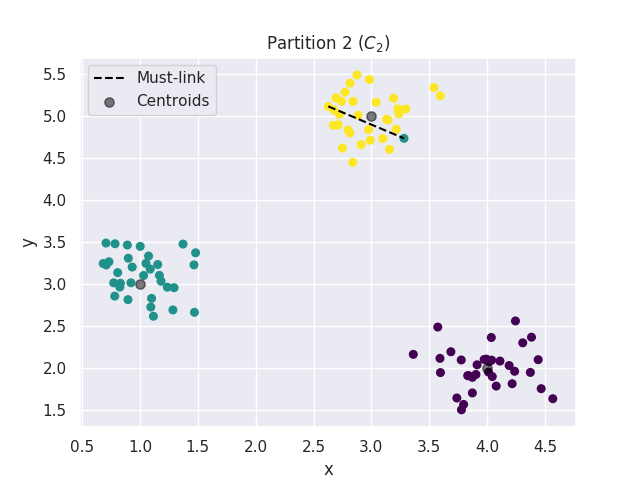
\includegraphics[width=.41\linewidth]{gfx/NewProp/SHADE/C2}} \quad
	\caption{Three partitions over a toy dataset.}
	\label{fig:toydatasets}
\end{figure}

Table \ref{tab:fitnessfunctions} shows the fitness values for each partition from Figure \ref{fig:toydatasets}. We refer to the function presented in Equation \eqref{eq1} as $f_1$ and to the function presented in Equation \eqref{eq14} as $f_2$.

\begin{table}[!h]
	\centering
	\setlength{\tabcolsep}{7pt}
	\renewcommand{\arraystretch}{1.3}
	%\begin{adjustwidth}{-1in}{-1in}
	\resizebox{\textwidth}{!}{
		\begin{tabular}{c c c c c c}
			\hline
			\multirow{2}{*}{Partition} &
			\multicolumn{2}{c}{Expression} &&
			\multicolumn{2}{c}{Value} \\
			\cline{2-3} \cline{5-6}
			& $f_1$ & $f_2$ && $f_1$ & $f_2$ \\
			\hline
			$C_0$ & $z_0$ & $z_0$ && $0.457$  & $0.457$  \\
			$C_1$ & $z_1$ & $z_1$ && $0.540$  & $0.540$  \\
			$C_2$ & $z_2 + (\mu * N * \text{infsblt})$ & $z_2 * (\text{infsblt} + 1)$  && $0.503 + 1000 = 1000.503$ &  $0.503 * 2 = 1.005$ \\
			\hline
			
	\end{tabular}}
	%\end{adjustwidth}
	
	\caption{Expression and value of fitness functions over three partitions ($\mu = 10$).}
	\label{tab:fitnessfunctions}
\end{table}

Results in Table \ref{tab:fitnessfunctions} are a clear example of the above. In the general case, by using $f_2$ the penalty for violating constraints is proportional to the within-cluster-sum-of-squares---the lower it is, the lower the penalty. This is not the case with $f_1$, whose penalty term is independent of the within-cluster-sum-of-squares, which can result in a difference of several orders of magnitude between partitions satisfying different amounts of constraints.

As in \cite{de2017comparison} we apply a local optimization procedure to the individuals of the population, but without transferring its results to the original individual in order to maintain diversity. The difference is that we do not apply it to the whole population but only to a number $P_e$ of individuals considered as the elite of the population, with the aim of preserving a good exploration-exploitation trade-off. The percentage of individuals considered as elite must be determined for each case. Figure \ref{fig:SHADE_CC} shows a representation of the \acs{SHADE}$_{CC}$ optimization process. Arrows in red indicate population sorting by fitness.

\begin{figure}[!h]
	\centering
	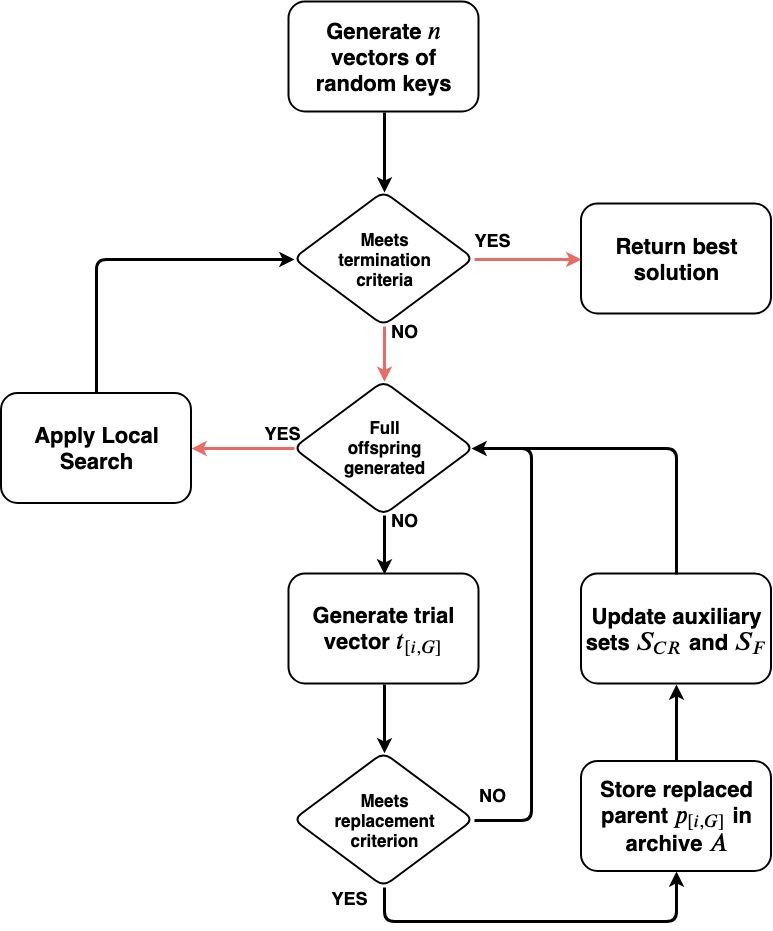
\includegraphics[scale=0.3]{gfx/NewProp/SHADE/SHADE_Diagram.jpg} 
	\caption{\acs{SHADE}$_{CC}$ optimization process for constrained clustering.}\label{fig:SHADE_CC}
\end{figure}

Algorithm \ref{alg:SHADE} describes the overall \acs{SHADE}$_{CC}$ optimization process, including the \acs{LS} procedure presented in Algorithm \ref{alg:SHADE_LS}. The goal of this procedure is to locally improve solutions (individuals from $P$) in a non-exhaustive way. To do so, it randomly choses an instance from the dataset and iteratively assigns it to different clusters. When improvement in the fitness function is detected, the change is transferred to the solution, when there is no possible improvement the local optimization process stops.

\begin{algorithm}
	\SetNlSty{textbf}{[}{]}
	\SetNlSkip{0.5em}
	\setstretch{1.2}
	\SetKwFunction{Sort}{Sort}
	\SetKwFunction{LocalSearch}{LocalSearch}
	\KwIn{Dataset $X$, constraint sets $C_=$ and $C_{\neq}$, population size $p_{size}$, elite size $P_e$, number of clusters $k$.}
	\tcp{Initialization phase}
	$G \leftarrow 0$\\
	Initialize population $P_0 \leftarrow \{p_{[1,0]}, \cdots, p_{[p_{size},0]}\}$\\
	Initialize all values in $M_{CR}$, $M_F$ to 0.5\\
	$A \leftarrow \emptyset$; $h \leftarrow 1$\\
	\tcp{Main loop}
	\While{Termination criteria are not met}{
		
		$S_{CR} \leftarrow S_F \leftarrow \emptyset$\\
		$P_G \leftarrow$ \Sort{$P_G$} \tcp{Sort the population}
		\tcp{Apply an LS procedure to the elite of the population}
		\LocalSearch{$\{p_{[1,G]}, \cdots, p_{[p_{e},G]}\}$}\\
		\For{$i \in [1,p_{size}]$}{
			$r_i \leftarrow$ randInt$[1,|M|]$\\
			$CR_{[i,G]} \leftarrow$ randn$_i(M_{[CR,r_i]}, 0.1)$\\
			$F_{[i,G]} \leftarrow$ randc$_i(M_{[F,r_i]}, 0.1)$\\
			$p_{[i,G]} \leftarrow$ rand$[N/2, 0.2]$\\
			Generate trial vector $t_{[i,G]}$ by current-to-$p$best/1/bin\\
			
			\eIf{$f(t_{[i,G]}) \le f(p_{[i,G]})$}{
				$p_{[i,G + 1]} \leftarrow t_{[i,G]}$
			}{
				$p_{[i,G + 1]} \leftarrow p_{[i,G]}$
			}
			
			\If{$f(t_{[i,G]}) < f(p_{[i,G]})$}{
				$p_{[i,G]} \rightarrow A$;
				$CR_{[i,G]} \rightarrow S_{CR}$;
				$F_{[i,G]} \rightarrow S_{F}$
			}
			
		}
		\tcc{Whenever $|A| > |P|$, randomly select an individual from $A$ to be deleted so that $|A| \le |P|$}
		\If{$S_{CR} \neq \emptyset$ \textbf{and} $S_{F} \neq \emptyset$}{
			Update $M_{[CR,h]}$ and $M_{[F,h]}$ based on $S_{CR}$ and $S_{F}$\\
			$h \leftarrow (h + 1) \mod |M|$
		}
		$G \leftarrow G + 1$
	}
	\caption{\acs{SHADE}$_{CC}$}\label{alg:SHADE}
\end{algorithm}

\newpage

\begin{algorithm}
	\SetNlSty{textbf}{[}{]}
	\SetNlSkip{0.5em}
	\setstretch{1.2}
	\SetKwFunction{RandomShuffle}{RandomShuffle}
	\SetKwRepeat{Do}{do}{while}
	\KwIn{Dataset $X$, constraint sets $C_=$ and $C_{\neq}$, decoded random-key vector (solution) $S$, number of clusters $k$.}
	\BlankLine
	\While{$improvement$}{
		$improvement \leftarrow$ \texttt{false} \\
		
		$s_i \leftarrow $ Select random object from $S$\\
		\tcp{Random shuffle labels set}
		$RSL \leftarrow $ \RandomShuffle{$\{1,\cdots,K\}$}\\
		\For{$l \in RSL$}{
			$S^\prime \leftarrow S$\\
			\tcp{Move object $s_i$ to the cluster associated with label $l$}
			$S^\prime$\texttt{[}$s_i$\texttt{]} $\leftarrow l$\\
			\If{$f(S^\prime) < f(S)$}{
				$S \leftarrow S^\prime$\\
				$improvement \leftarrow$ \texttt{true} \\
			}
		}
	}
	\BlankLine
	\KwRet{$S$}
	
	\caption{\acs{SHADE}$_{CC}$ Local Search}\label{alg:SHADE_LS}
\end{algorithm}

\section{Constrained Clustering Through Local Search} \label{sec:DILS}

Following the stream of thought introduced at the beginning of this chapter, it is justified to think that metaheuristics constitute a promising approach to find approximate quality solutions to the tough challenge that constrained clustering represents. Metaheuristic algorithms are designed to explore the solution space of a problem with the guidance of a fitness (heuristic) function \cite{Gendreau:2010:HM:1941310}. In this type of approaches the key is to find a good exploration-exploitation tradeoff. This is the reason why the classic \acf{LS} heuristic algorithm derived in the \acf{ILS} metaheuristic algorithm, which introduces periodic perturbations in the exploration of the solution space to escape local optima \cite{lourencco2010iterated}. \acs{ILS} (or variants of it) has been applied to a wide variety of problems, including the traveling salesman \cite{archetti2018iterated}, the quadratic multiple knapsack \cite{avci2017multi} or the vehicle routing problem \cite{chentli2018impact, estrada2019biased}. \acs{ILS} is also very commonly used in the design of hybrid methods with good exploration-exploitation tradeoff, such as its combination with expediting mechanisms \cite{zohali2019reformulation} or with the success history based differential evolution algorithm \cite{zhao2019hybrid}. In this section we propose a new variant of the \acs{ILS} method, the \acs{DILS}, which introduces diversity in the exploration of the solution space in an adaptive and guided way.

\subsection{A Glimpse into Iterated Local Search}

Before defining \acs{ILS}, it is necessary to understand \acs{LS} and the motivation behind the design of methods with greater exploratory capabilities.

\acs{LS} is a procedure that consists in performing an heuristics-guided iterative improvement. With a valid solution to the problem as an initial state, \acs{LS} uses a neighbor generation operator to explore new solutions. The current solution is replaced when a better one is found. In order to evaluate solutions, a function to assess their suitability, known as \textit{fitness function}, is used. Ideally, the closer a solution is to the global optimum, the better its fitness value will be.

Both the neighbor generation operator and the fitness function used by \acs{LS} must be defined for each particular problem. The fitness function $f(\cdot)$ determines how good the solution achieved is with respect to the purpose of the problem. The neighbor generation operator attempts to improve upon a solution $S$ to the problem by modifying a few of its components, and thus generating a new solution $S^\prime$.

The Algorithm \ref{alg:BasicLS} presents a basic scheme for an \acs{LS} procedure. It is worth noting that the condition of line 4 must be adapted depending on whether the problem to be solved is one of maximization or minimization. In addition, the general scheme assumes that the optimization process ends when the current solution is not improved. However, the stop condition can be adapted to each problem.

\begin{algorithm}
	\SetNlSty{textbf}{[}{]}
	\SetNlSkip{0.5em}
	\setstretch{1.2}
	\SetKwFunction{GenerateNeighbor}{GenerateNeighbor}
	\SetKwRepeat{Do}{do}{while}
	\KwIn{Initial solution $S$}
	\BlankLine
	\While{$improvement$}{
		$improvement \leftarrow$ \texttt{false} \\
		
		$S^\prime \leftarrow $ \GenerateNeighbor{$S$}
		
		\If{$f(S^\prime) < f(S)$}{
			
			$S \leftarrow S^\prime$\\
			$improvement \leftarrow$ \texttt{true} \\
			
		}	
	}
	\BlankLine
	\KwRet ($S$)
	
	\caption{Basic Local Search}\label{alg:BasicLS}
\end{algorithm}

With \acs{LS} defined in this way, it is easy to see that the solution achieved will be the local optimum $S^*$ that is closest to the initial solution $S$. Figure \ref{img:LS} shows a pictorial representation of the above.

\begin{figure}[!h]
	\centering
	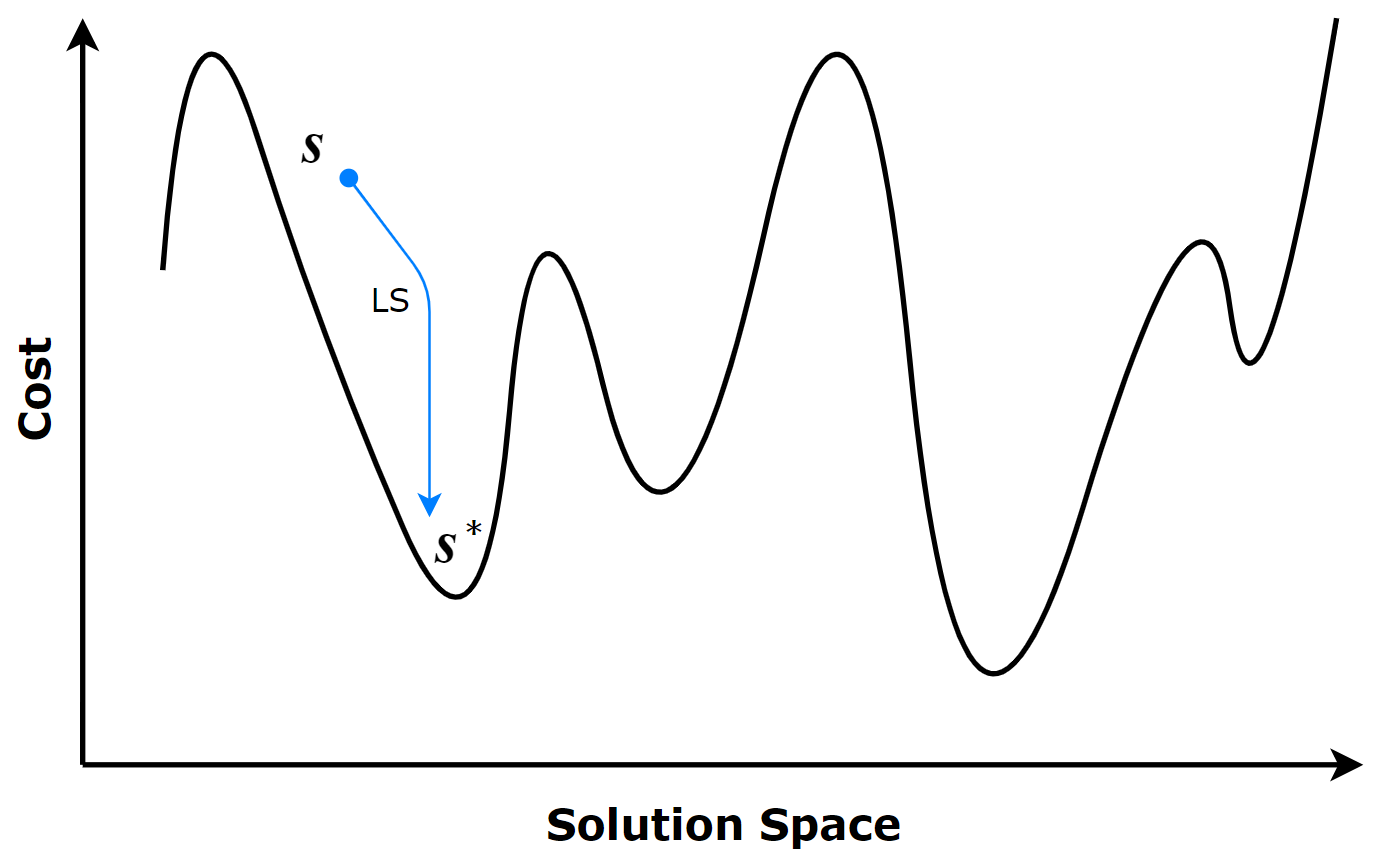
\includegraphics[scale=0.25]{gfx/NewProp/DILS/LS.png}
	\caption{Local optimum achieved by an \acs{LS} procedure.}\label{img:LS}
\end{figure}

It is therefore necessary to turn to techniques that introduce diversity in the search procedure to avoid the problem of local optimum. This is exactly what \acs{ILS} is trying to do. With \acs{ILS}, once we have reached a local optimum $S^*$, we apply a perturbation to it that will result in a new solution $S^\prime$. With a high probability, $S^\prime$ will not be another local optimum and instead will be far enough away from $S^*$. After that, we will apply an \acs{LS} procedure to find a new local optimum $S^{*\prime}$. Figure \ref{img:ILS} shows a representation of the aforementioned concepts.

\begin{figure}[!h]
	\centering
	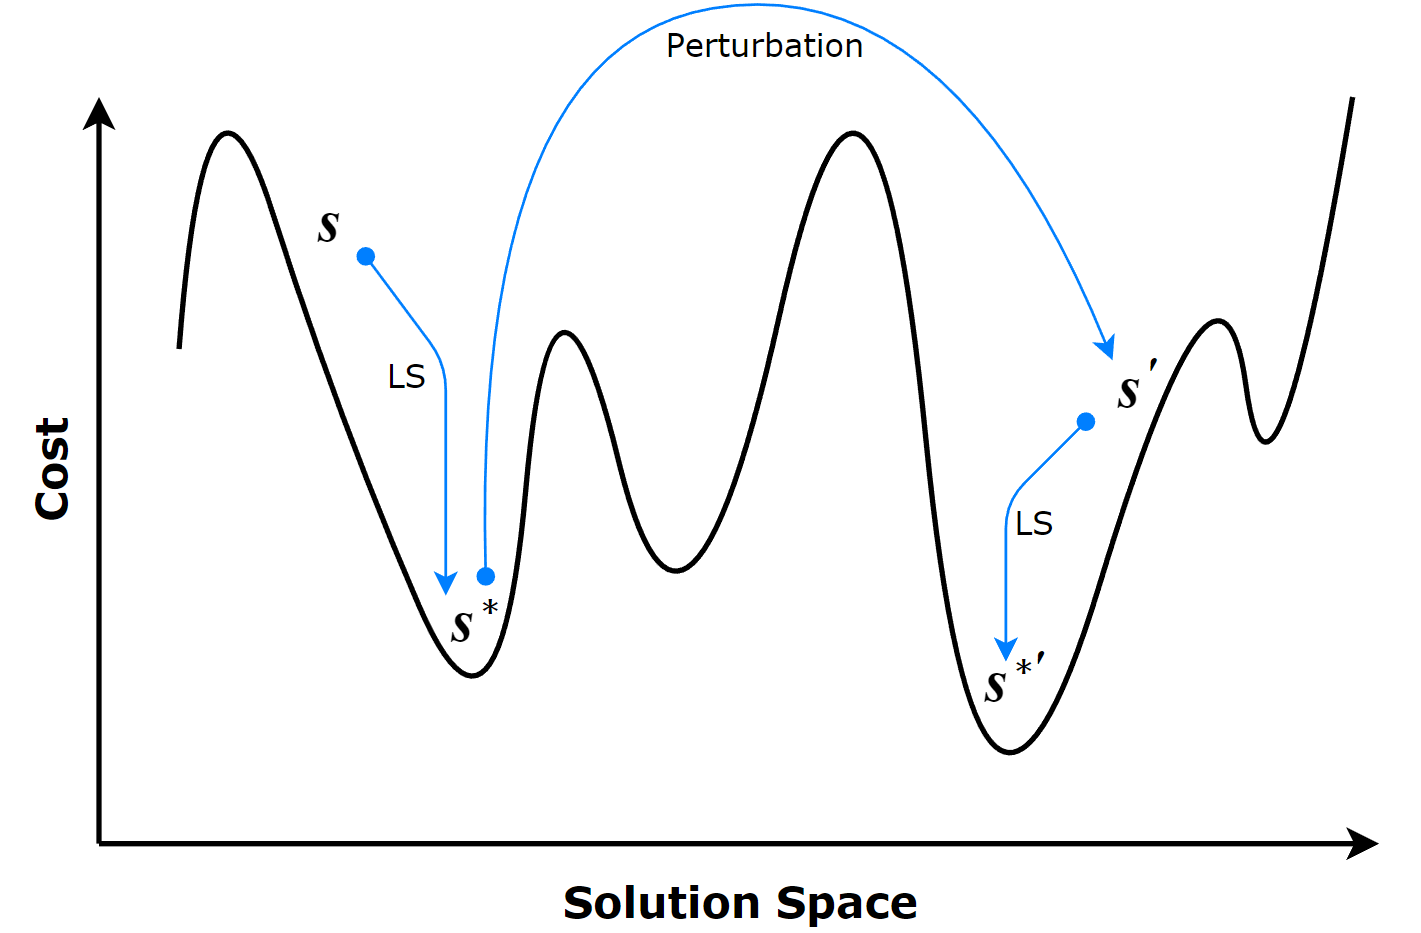
\includegraphics[scale=0.25]{gfx/NewProp/DILS/ILS.png}
	\caption{\acs{ILS} perturbation over an \acs{LS} local optimum.}\label{img:ILS}
\end{figure}

It should be noted that, if the perturbation applied to $S*$ is too small, most likely the local optimum closest to $S^\prime$ is again $S^*$ and therefore the exploration of the solution space is not be effective. On the other hand, if the perturbation is too big, there will be no bias in the generation of new solutions, and therefore the procedure becomes a random-reboot method.

The generation of perturbations for the local optimum $S^*$ may vary depending on the problem, and may be based on previous solutions. In this way, it is possible to keep a history of solutions reached so far, so they can be used when applying the perturbation. Algorithm \ref{alg:ILS} summarizes the overall optimization process of \acs{ILS}.

\begin{algorithm}
	\SetNlSty{textbf}{[}{]}
	\SetNlSkip{0.5em}
	\setstretch{1.2}
	\SetKwFunction{LocalSearch}{LocalSearch}
	\SetKwFunction{Perturbation}{Perturbation}
	\SetKwRepeat{Do}{do}{while}
	\KwIn{Initial solution $S$}
	\BlankLine
	$S^* \leftarrow$ \LocalSearch{$S$}\\
	\While{Termination criteria are not met}{
		
		$S^\prime \leftarrow $ \Perturbation{$S^*$, $history$}\\
		$S^{*\prime} \leftarrow$ \LocalSearch{$S^\prime$}
		
		\If{$f(S^{*\prime}) < f(S^*)$}{
			
			$S^* \leftarrow S^{*\prime}$
			
		}	
	}
	\BlankLine
	\KwRet ($S*$)
	
	\caption{Basic Iterated Local Search}\label{alg:ILS}
\end{algorithm}

In the \acs{ILS} scheme described in Algorithm \ref{alg:ILS} the acceptance criterion only uses the difference in the cost of the compared solutions to choose between them. This is the simplest scheme and does not rely on the history of previous solutions.

\subsection{The Dual Iterative Local Search Method}

The Dual Iterative Local Search (DILS) is a new variant of the classic ILS method. Its goal is to perform a search in the solution space to find the solution with the best fitness value (given by fitness function $f$) by introducing diversity in an adaptive and guided way. While ILS works with a single individual, DILS keeps two of them $\{m_b, m_w\}$ in memory at all times, which allows it to guide diversity-inducing methods and to avoid local optima. The individual $m_b$ is the one providing the best fitness value, whereas $m_w$ provides the worst fitness value at the end of each stage (generation) of the optimization process.

In each generation $G$ of the optimization process DILS builds a new individual by applying a recombination operator to $m_b$ and $m_w$. After that, it applies a strong mutation operator to the newly generated individual. This is the individual DILS applies the LS procedure to in order to improve its fitness value, resulting in the trial individual $m_t$. The trial individual $m_t$ replaces the worst of its predecessors, $m_w$, if it achieves a better fitness value; this operation represents the acceptance criterion for DILS. Equation \ref{eq1.2} displays the expression for this criterion in the case of a minimization problem.

\begin{equation}
m_{w,G} = \left\{ \begin{array}{lc}
m_t &   \text{if} \;\; f(m_t) < f(m_w)\\
m_{w,G} &  \text{otherwise}
\end{array}
\right..
\label{eq1.2}
\end{equation}

Now, the process described so far will most likely fall into a local optimum, effectively stopping the exploration of the solution space. To avoid it DILS implements a reinitialization method for $m_w$ based on the difference between the two individuals it keeps in memory ($\{m_b, m_w\}$). Equation \ref{eq2.2} shows the reinitialization criterion for a minimization problem. RandInit$()$ is a function that returns a randomly initialized individual and $\xi \in [-1,1]$ is the parameter that controls the tolerance of the reinitialization method.

\begin{equation}
\resizebox{0.85 \textwidth}{!}{$
	m_{w,G+1} = \left\{ \begin{array}{lc}
	\text{RandInit}() &   \text{if} \;\; f(m_b) - f(m_w) > f(m_b) * \xi \;\;\\
	m_{w,G} &  \text{if} \;\; f(m_b) - f(m_w) \le f(m_b) * \xi \; \wedge \; f(m_b) < f(m_w) \;\;\\
	m_{b,G} &  \text{if} \;\; f(m_b) - f(m_w) \le f(m_b) * \xi \; \wedge \; f(m_b) > f(m_w) \;\;\\
	\end{array}
	\right.$}.
\label{eq2.2}
\end{equation}

To maintain consistency between generations we also need to reassign $m_b$ to the true best individual once the reinitialization criterion has been tested, Equation \ref{eq5.2} formalize this simple step. This way the best individual is always preserved and therefore always takes part in the process of generating new individuals (via the recombination operator) as the best predecessor.

\begin{equation}
m_{b,G+1} = \left\{ \begin{array}{lc}
m_{b,G} &  \text{if} \;\; f(m_b) < f(m_w) \;\;\\
m_{w,G} &  \text{if} \;\; f(m_b) > f(m_w) \;\;\\
\end{array}
\right..
\label{eq5.2}
\end{equation}

Figure \ref{img:DILS_diag} summarizes the DILS optimization process. Arrows in red indicate stages of the algorithm where $m_b$ and $m_w$ are reassigned to the true best and worst individual respectively. This way, at the point where the reinitialization criterion is tested, it is possible for $f(m_w)$ to yield a smaller value than $f(m_b)$, so that $f(m_b) - f(m_w)$ can be either positive or negative. 

\begin{figure}[!h]
	\centering
	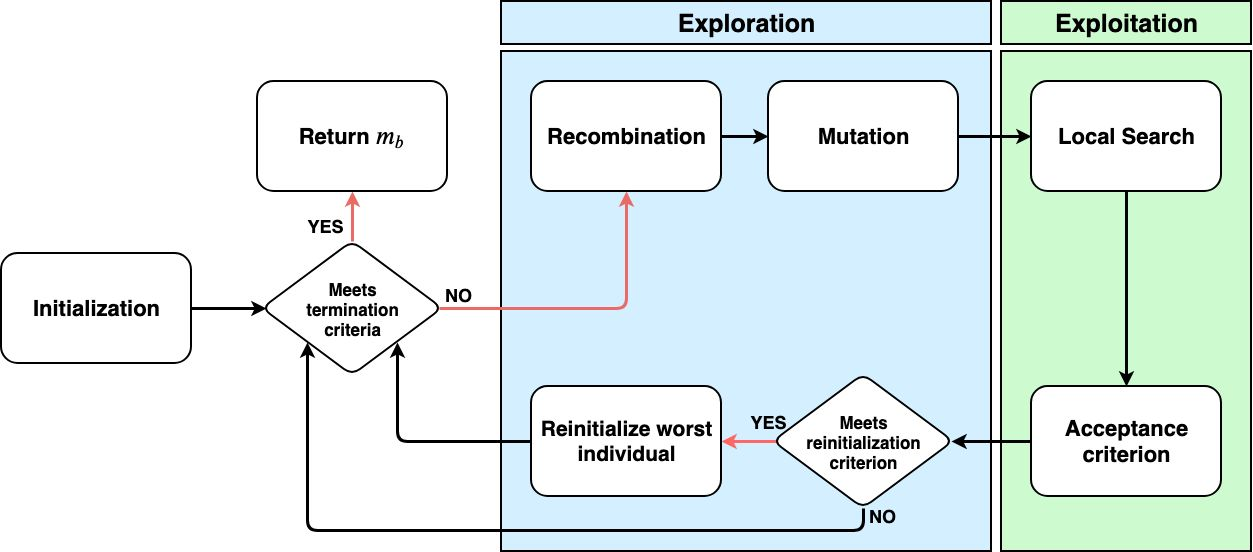
\includegraphics[scale=0.25]{gfx/NewProp/DILS/DILSDiagram.jpg}
	\caption{Diagram summarizing DILS optimization process.}\label{img:DILS_diag}
\end{figure}

This highlights the influence of the parameter $\xi$. Let us assume again a minimization problem. On one hand, if $\xi > 0$, then the true worst individual is only reinitialized when $m_t$ replaces $m_w$ and is also better than $m_b$ by a margin. On the other hand, if $\xi < 0$, we allow DILS to reinitialize the true worst individual even when $m_t$ is not better than $m_b$. It becomes clear that when $\xi = 0$ the worst individual is restarted if $f(m_b) = f(m_w)$. Note that $\xi$ could take any real value, but it is not realistic to set it outside of the range $[-1,1]$, and we recommend $[-0.5, 0.5]$. To summarize, the closer $\xi$ is to 1 the more restrictive the reinitialization criterion is---in the minimization case. It is also worth noting that in early stages of the optimization process the reinitialization criterion tends to be met more often than in later stages. The reason for this is that the fitness value of the best individual $f(m_b)$ never worsens ($f(m_{b,G}) \ge f(m_{b,G+1})$), so it becomes increasingly harder for $m_w$ to achieve similar or better scores. Algorithm \ref{alg:DILS} summarizes the overall DILS optimization process.

\newpage

\begin{algorithm}
	\SetNlSty{textbf}{[}{]}
	\SetNlSkip{0.5em}
	\setstretch{1.1}
	\SetKwFunction{RandInit}{RandInit}
	\SetKwFunction{Best}{Best}
	\SetKwFunction{Worst}{Worst}
	\SetKwFunction{Recombination}{Recombination}
	\SetKwFunction{Mutation}{Mutation}
	\SetKwFunction{LocalSearch}{LocalSearch}
	\KwIn{Probability for recombination operator $p_r$, segment size for mutation operator $p_s$, reinitialization method tolerance $\xi$.}
	\tcp{Initialization phase}
	$G \leftarrow 0$\\
	$m_b \leftarrow$ \RandInit{};
	$m_w \leftarrow$ \RandInit{}\\
	\tcp{Main loop}
	\While{Termination criteria are not met}{
		\tcp{Find best and worst individual}
		$m_b \leftarrow $ \Best{$ \{m_b, m_w\} $};
		$m_w \leftarrow $ \Worst{$ \{m_b, m_w\} $}\\
		\tcp{Generate new individual}
		$m_t \leftarrow $ \Recombination{$m_b, \; m_w$}\\
		$m_t \leftarrow $ \Mutation{$m_t$}\\
		\tcp{Improve new individual}
		$m_t \leftarrow $ \LocalSearch{$m_t$}\\
		\tcp{Apply replacement operator}
		\If{$f(m_t) < f(m_w)$}{
			
			$m_w \leftarrow m_t$\\
			
		}
		\tcp{Check restart criterion}
		\If{$f(m_b) - f(m_w) > f(m_b) \times \xi$}{
			
			$m_b \leftarrow $ \Best{$ \{m_b, m_w\} $}\\
			$m_w \leftarrow$ \RandInit{}\\
			
		}
		
		$G \leftarrow G + 1$
	}
	
	$m_b \leftarrow $ \Best{$ \{m_b, m_w\} $}\\
	\KwRet{$m_b$}
	\caption{\acs{DILS}}\label{alg:DILS}
\end{algorithm}

For the recombination and mutation operators that appear in Algorithm \ref{alg:DILS}, we use the uniform recombination and the segment mutation operator respectively. The uniform recombination consists in selecting features from the best individual $m_b$ based on a given probability $p_r$ to introduce them in the resulting individual, so the rest of the features are taken from $m_w$ \cite{spears1995virtues}. The segment mutation operator consists in replacing a fixed-size segment from the features of the individual with randomly generated features. The size of the segment $p_s$ must be fixed at the beginning of the optimization process.

It should be noted that the optimization process described so far is applicable to any minimization problem, although it is clear that there is a direct adaptation of \acs{DILS} for maximization problems. In addition, the \acs{LS} procedure used to obtain the trial individual $m_t$ must be specified for each problem, as well as numerical representation details and termination criteria.

\subsection[\acsfont{DILS} Optimization Scheme for Constrained Clustering]{DILS Optimization Scheme for Constrained Clustering} \label{sec:DILS_CC}

In this section, we present the application scheme of \acs{DILS} to constrained clustering. We will call this new approach \acs{DILS}$_{CC}$. We will use an integer-based representation for all the individuals \acs{DILS}$_{CC}$ work with; this way, each individual $m$ is defined as a vector of $n$ integers---with $n$ being the number of instances of the dataset. Each integer $m_i \in [0,k)$ in $m$ represents the label of the cluster that instance $x_i$ is assigned to, and therefore each individual $m$ is a solution to the clustering problem. Additionally, in order not to bias the exploration of the solution space, we will use random initialization to set $m_b$ and $m_w$; this procedure will also be used in the reinitialization of $m_w$. Regarding the fitness function $f(\cdot)$, for each individual $m$ its fitness value $f(m)$ can be calculated as in Equation \ref{eq14}.

We also need to specify an \acs{LS} procedure for \acs{DILS} to be able to improve the mutant individual to obtain the trial vector $m_t$. Algorithm \ref{alg:DISL_LS} shows the \acs{LS} used in \acs{DILS}$_{CC}$. Note that, in order not to bias the search, indices from vector $m$ and labels from the set of labels are randomly chosen to generate a random subset of the neighborhood of $m$. This \acs{LS} procedure is similar to the one presented in Algorithm \ref{alg:SHADE_LS}, being the mos relevant difference the introduction of the maximum number of neighbors $p_m$ that can be generated in each call; this is done to ensure a better exploration-exploitation tradeoff. 

\begin{algorithm}
	\SetNlSty{textbf}{[}{]}
	\SetNlSkip{0.5em}
	\setstretch{1.1}
	\SetKwFunction{RandomShuffle}{RandomShuffle}
	\SetKwFunction{Rand}{Rand}
	\SetKwRepeat{Do}{do}{while}
	\KwIn{Dataset $X$, constraint sets $C_=$ and $C_{\neq}$, individual (solution) $S$, number of clusters $k$, maximum number of neighbors that can be generated $p_m$.}
	\BlankLine
	\While{$improvement$ {\bf and} $generated < p_m$}{
		$improvement \leftarrow$ \texttt{false} \\
		\tcp{Select random index (object) from $S$}
		$i \leftarrow $ \Rand{$1$,$n$} \\
		\tcp{Random shuffle labels set}
		$RSL \leftarrow $ \RandomShuffle{$\{1,\cdots,K\}$}\\
		\For{$l \in RSL$}{
			$S^\prime \leftarrow S$\\
			\tcc{Move object $i$ from $S$ to the cluster associated with label $l$}
			$S^\prime_i \leftarrow l$\\
			\If{$f(S^\prime) < f(S)$}{
				$S \leftarrow S^\prime$\texttt{;} $improvement \leftarrow$ \texttt{true} \\
			}
			$generated \leftarrow generated + 1$\\
		}
	}
	\BlankLine
	\KwRet{$S$}
	
	\caption{\acs{DILS}$_{CC}$ Local Search}\label{alg:DISL_LS}
\end{algorithm}


















